\chapter{Exponential Functions}
%%%%%%%%%%%%%%%%%%%%%%%%%%%%%%%%%%%%%%%%%%%%%
\section{Exponential and Logarithmic Functions}
Laws of logarithms. This will be covered in detail in Chapter 4.\\
$\log _{a} X Y =\log _{a} X +\log _{a} Y$ 

$\log _{a} \genfrac{(}{)}{}{}{X}{Y} =\log _{a} X -\log _{a} Y$ 

$\log _{a} X^{n} =n \log _{a} X$ 


\section{$e^x$}
We defined $a^{x}$ where $a >0$ in chapter 1, however $x$ was restricted to rational numbers. We now want to explore $a^{x}$ where $a >0$ and $x$ is any real number. 

We can show that values exist simply by pressing buttons on the calculator or drawing
a graph using Desmos, however an intuitive understanding can be obtained by considering appropriate values. 

Consider $2^{\pi }$. We know $\pi  =3.141592654 \ldots $. $2^{\pi }$ should be between $2^{3}$\ and $2^{4}$. That is between $8$ and $16$. We can evaluate 

\qquad \qquad \qquad \qquad \qquad \qquad \qquad \qquad
\begin{tabular}[c]{ll}$2^{3.1}$  & $8.5741877$  \\
$2^{3.14}$  & $8.815240927$  \\
$2^{3.141}$  & $8.821353305$  \\
$2^{3.1415}$  & $8.824411082$  \\
$2^{3.14159}$  & $8.824961595$  \\
$2^{3.141592}$  & $8.824973829$  \\
$2^{3.1415926}$  & $8.824977499$  \\
$2^{3.14159265}$  & $8.824977805$  \\
$2^{3.141592654}$  & $8.82497783$
\end{tabular}

We could continue this process. If
we enter $2^{\pi }$ on the calculator the answer obtained is
\begin{equation*}2^{\pi } =8.824977827
\end{equation*}

The graph of $y =2^{x}$, $ \forall x \in \mathbb{R}$ is shown. 

   
\setlength\fboxrule{0.01in}\setlength\fboxsep{0.2in}\fcolorbox[HTML]{000000}{FFFFFF}{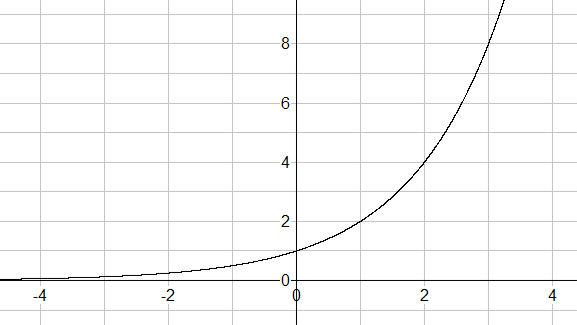
\includegraphics[ width=3.7758in, height=2.1378in,]{L4SZ282M}
}


Recall $y =f (x)$ is a function and $y =f ( -x)$ is the same function with every $x$ replaced with $ -x$, i.e. $y =f ( -x)$ is the reflection of $y =f (x)$ in the $y$-axis. 

If $y =2^{x}$ then $y =2^{ -x}$ is the reflection of $y =2^{x}$ in the $y$-axis. But $y =2^{ -x} =\left (2^{ -1}\right )^{x} =\genfrac{(}{)}{}{}{1}{2}^{x}$. 

\subsubsection{Graphing Exercise}
Use Desmos to verify that $y =2^{ -x}$ and $y =\genfrac{(}{)}{}{}{1}{2}^{x}$ are the same. 

%Here are the graphs of $y =2^{x}$ and $y =2^{ -x}$. 

   
%\setlength\fboxrule{0.01in}\setlength\fboxsep{0.2in}\fcolorbox[HTML]{000000}{FFFFFF}{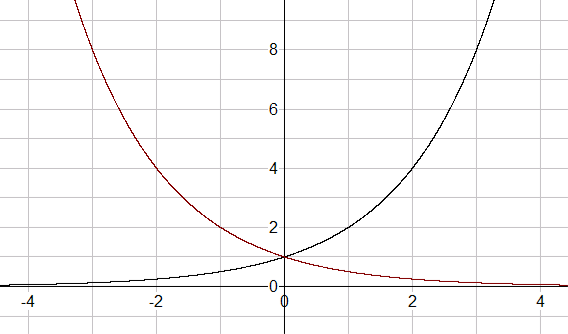
\includegraphics[ width=3.7265in, height=2.2027in,]{L4SZ282N}
%}


\subsection{The Exponential Function $f (x) =a^{x}$}
Let $y =a^{x}$ where $a >0$ 


\begin{tabular}[c]{|l|c|l|}\hline
When $0 <a <1$  & $y =a^{x}$ looks like  &    
\setlength\fboxrule{0in}\setlength\fboxsep{0.2in}\fcolorbox[HTML]{000000}{FFFFFF}{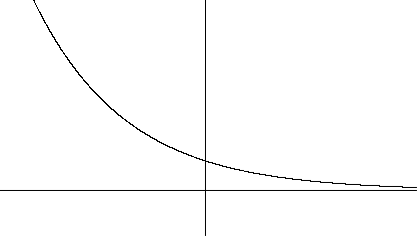
\includegraphics[ width=1.9086in, height=1.0853in,]{L4SZ282O}
}
\\
\hline
When $a =1$  & $y =a^{x} =1^{x} =1$ looks like  &    
\setlength\fboxrule{0in}\setlength\fboxsep{0.2in}\fcolorbox[HTML]{000000}{FFFFFF}{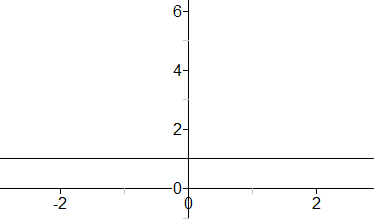
\includegraphics[ width=1.9095in, height=1.1234in,]{L4SZ282P}
}
\\
\hline
When $a >1$  & $y =a^{x}$ looks like  &    
\setlength\fboxrule{0in}\setlength\fboxsep{0.2in}\fcolorbox[HTML]{000000}{FFFFFF}{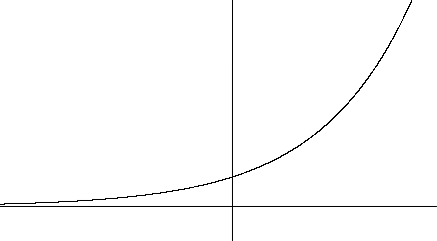
\includegraphics[ width=1.9372in, height=1.0741in,]{L4SZ282Q}
}
\\
\hline
\end{tabular}

$f (x) =a^{x}$ is called an \emph{exponential} function. $a$ is called the \emph{base} of the exponential function. The domain
is $\mathbb{R}$. the range is $\left (0 ,\infty \right )$. The $x$-axis is an asymptote. 

\subsubsection{Example 1}
Find the equation of the exponential function that passes through $\left (0 ,1\right )$ and $\left (3 ,125\right )$. 

Solution: An
exponential function that passes through $\left (0 ,1\right )$ is of the form $f (x) =a^{x}$. As $f (3) =125$ we substitute $x =3$ and get
\begin{align*}a^{3} &  = 125 \\
a &  = \sqrt[{3}]{125} =5\end{align*}

\subsection{Transformations of Exponential Functions}
Recall the transformations we have met so far 


\begin{tabular}[c]{ll}Vertical stretch of $a$  & $y =f (x) \leadsto y =a f (x)$  \\
Horizontal stretch of $\frac{1}{b}$  & $y =f (x) \leadsto y =f (b x)$  \\
Vertical shift of $c$ $\uparrow $  & $y =f (x) \leadsto y =f (x) +c$  \\
Horizontal shift of $d$ $ \longrightarrow $  & $y =f (x) \leadsto y =f (x -d)$  \\
Reflection in $x$-axis  & $y =f (x) \leadsto y = -f (x)$  \\
Reflection in $y$-axis  & $y =f (x) \leadsto y =f ( -x)$
\end{tabular}

Each of these transformations can be applied to an exponential
function. 

Given $y =2^{x}$ apply the following transformations. Draw a sketch showing where the graph crosses the
$y$-axis, its shape, its asymptote and one other point it passes through. 


\columnseprule =0.4pt
\begin {multicols}{2}

\begin{enumerate}
\item Horizontal shift of $ +2\vspace{+2.000000cm}$ 

\item Vertical shift of $ -3\vspace{+2.000000cm}$ 

\item Horizontal stretch of $2\vspace{+2.000000cm}$ 

\item Vertical stretch of $4\vspace{+2.000000cm}$ 

\item Horizontal stretch of $\frac{1}{3}\vspace{+2.000000cm}$ 

\item Vertical stretch of $\frac{1}{2}\vspace{+2.000000cm}$ 

\item Reflection in the x-axis\vspace{2cm}


\item Reflection in the y-axis\vspace{2cm} 

\item (Challenge) Reflection in $y = -1\vspace{+2.000000cm}$ 

\item (Challenge) Reflection in $x =1\vspace{+2.000000cm}$ \end{enumerate}

\end {multicols}

\subsection{The Natural Exponential Function}
The \emph{natural exponential function} has wide application in mathematics and is a particular example of the exponential
function. We have defined $f (x) =a^{x}$ and there is a particular value of $a$ that we denote by the letter $e$. This will turn up again and again in future courses and later it will be carefully
defined for you. In this course we will meet some of the applications that use $e$. $e$ is an irrational number (like $\pi $, $\sqrt{2}$ etc.). It can be found on the calculator and to 20 decimal places it is
\begin{equation*}e \approx 2.71828182845904523536
\end{equation*}

The natural exponential function $f (x) =e^{x}$ is often simply referred to as the exponential function. 

\subsubsection{Example 2}
Use your calculator to evaluate to 5dp 


\begin{description}
\item [(a)] $e^{4}$ 

\item [(b)] $2 e^{ -0.7}$ 

\item [(c)] $e^{3.1}$ 

\item [(d)] $e^{e}$ \end{description}

($54.59815$, $0.99317$, $22.19795$, $15.15426$) 

\subsection{Exercise 1}
Use Desmos to sketch: 

\begin{description}
\item [(a)] $f (x) =e^{ -x}$ 

\item [(b)] $g (x) =2 e^{0.1 x}$ 

\item [(c)] $h (x) = -2.1 e^{ -0.12 x}$ \end{description}

\subsection{Exercise 2}
The exponential function can be used to model the way populations grow and diseases spread. The following
example is about the spread of an infectious disease in a small city whose population is $10,000$. After $t$ days the number of people who have caught the disease is modelled by the function
\begin{equation*}f (t) =\frac{10000}{5 +2495 e^{ -0.84 t}}
\end{equation*}


\begin{description}
\item [(a)] How many people had the disease initially? 

\item [(b)]
How many people have the disease after $1$ day? 

\item [(c)] How many people
have the disease after $5$ days? 

\item [(d)] Use Desmos
to graph the function. 

\item [(e)] Describe the behaviour
of the function. \end{description}

The graph has distinctive characteristics. It
starts at a particular nonzero value (when $t =0$) and increases slowly at first then more rapidly. It slows down after a time and
levels off because the exponential function in the denominator $ \leadsto 0$ when $t \leadsto \infty $. Graphs with these characteristics are called logistic curves. The
particular model is called a logistic growth model. 

\subsection{Exercises}
Find the exponential function $f (x) =a^{x}$ whose graph is given. 


\begin{tabular}[c]{ll}9.  & 10.
\\
   
\setlength\fboxrule{0.01in}\setlength\fboxsep{0.2in}\fcolorbox[HTML]{000000}{FFFFFF}{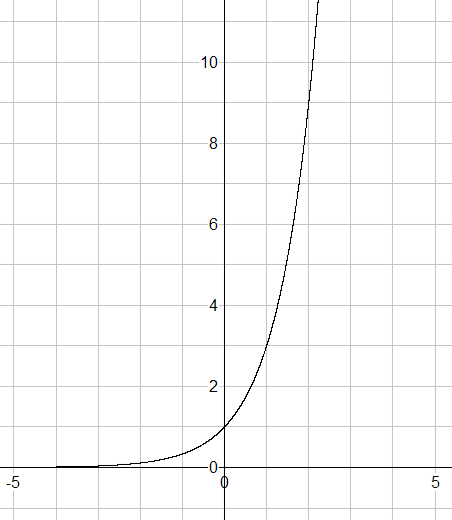
\includegraphics[ width=2.3047in, height=2.6472in,]{L4SZ282R}
}
&    
\setlength\fboxrule{0.01in}\setlength\fboxsep{0.2in}\fcolorbox[HTML]{000000}{FFFFFF}{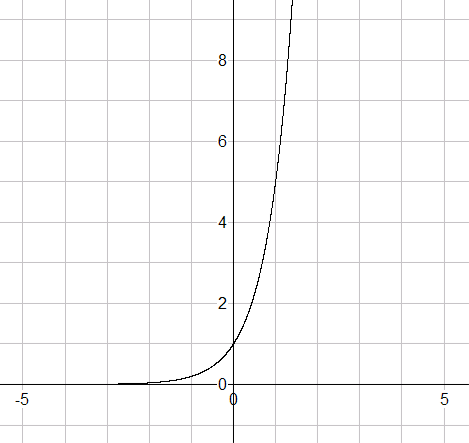
\includegraphics[ width=2.7164in, height=2.5676in,]{L4SZ282S}
}
\\
11.  & 12.  \\
\setlength\fboxrule{0.01in}\setlength\fboxsep{0.2in}\fcolorbox[HTML]{000000}{FFFFFF}{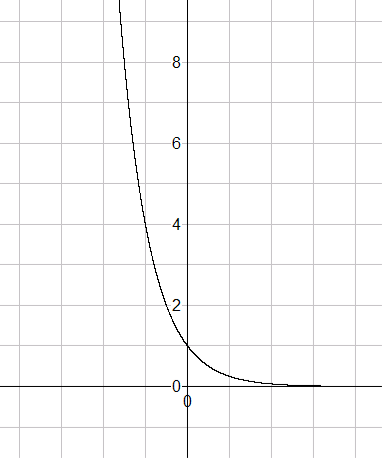
\includegraphics[ width=2.207in, height=2.6394in,]{L4SZ282T}
}
&    
\setlength\fboxrule{0.01in}\setlength\fboxsep{0.2in}\fcolorbox[HTML]{000000}{FFFFFF}{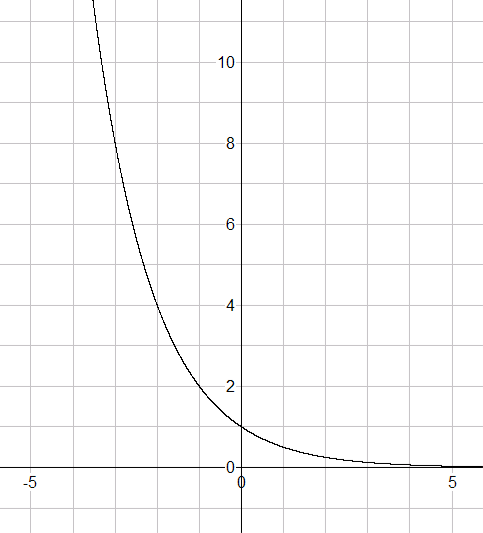
\includegraphics[ width=2.3938in, height=2.6385in,]{L4SZ282U}
}
\end{tabular}

For the following questions draw the graph of the function by transforming the given graph. State the domain, range and asymptote.  

\begin{tabular}[c]{ll}19. The given graph is $y =3^{x}\text{.}$ Draw $y = -3^{x}\vspace{+0.200000cm}$  & 21. The given graph is $y =2^{x}\text{.}$\ Draw $y =2^{x} -3$  \\
   
\setlength\fboxrule{0.01in}\setlength\fboxsep{0.2in}\fcolorbox[HTML]{000000}{FFFFFF}{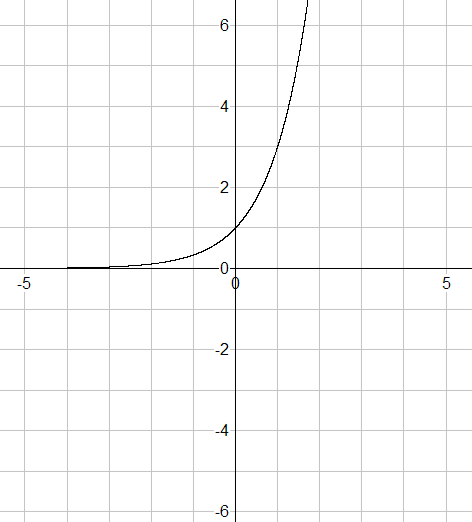
\includegraphics[ width=2.1594in, height=2.1851in,]{L4SZ282V}
}
\vspace*{0.5cm}  &    
\setlength\fboxrule{0.01in}\setlength\fboxsep{0.2in}\fcolorbox[HTML]{000000}{FFFFFF}{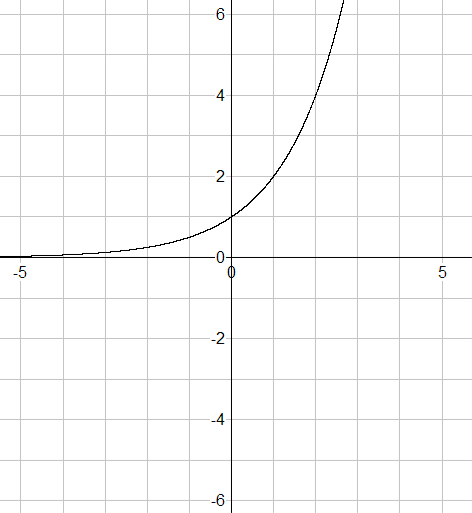
\includegraphics[ width=2.1793in, height=2.1679in,]{L4SZ282W}
}
\\
23. The given graph is $y =\frac{1}{2}^{x}\text{.}$ Draw $y =4 +\frac{1}{2}^{x}\vspace{+0.200000cm}$  & 25. The given graph is $y =10^{x}\text{.}$ Draw $y =10^{x +3}$  \\
   
\setlength\fboxrule{0.01in}\setlength\fboxsep{0.2in}\fcolorbox[HTML]{000000}{FFFFFF}{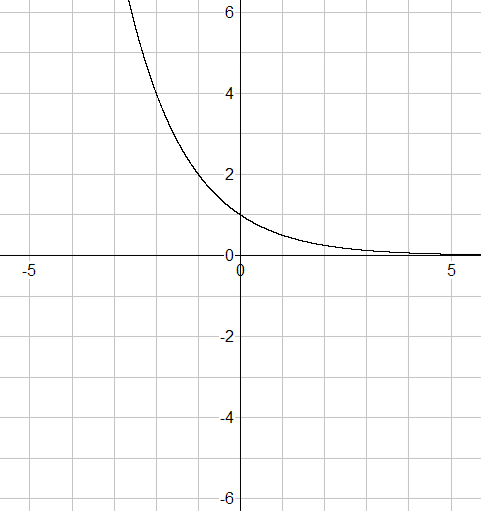
\includegraphics[ width=2.271in, height=2.2111in,]{L4SZ282X}
}
\vspace*{0.5cm}  &    
\setlength\fboxrule{0.01in}\setlength\fboxsep{0.2in}\fcolorbox[HTML]{000000}{FFFFFF}{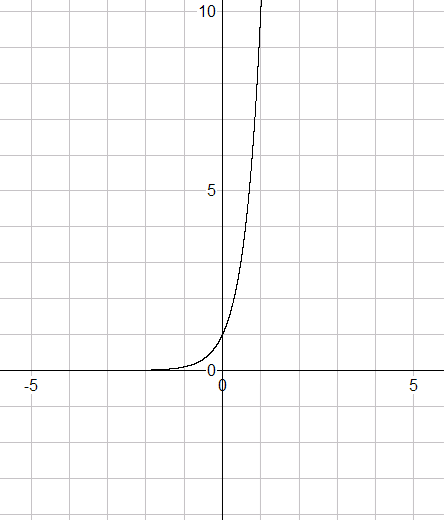
\includegraphics[ width=2.0496in, height=2.1964in,]{L4SZ282Y}
}
\\
27. The given graph is $y =e^{x}\text{.}$ Draw $y = -e^{x}\vspace{+0.200000cm}$  & 29. The given graph is $y =e^{ -x}\text{.}$ Draw $y =e^{ -x} -1$  \\
   
\setlength\fboxrule{0.01in}\setlength\fboxsep{0.2in}\fcolorbox[HTML]{000000}{FFFFFF}{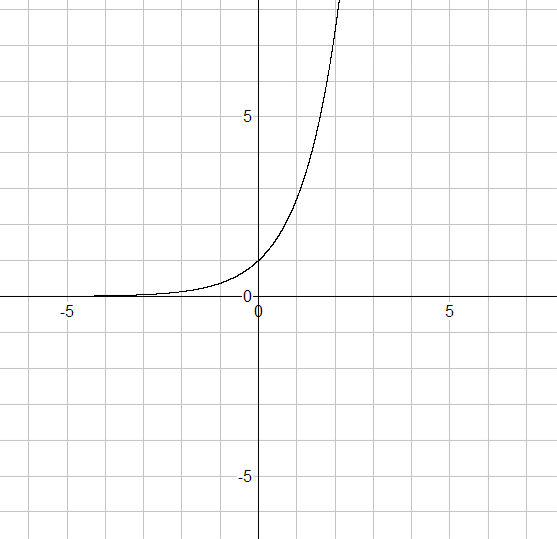
\includegraphics[ width=2.5114in, height=2.1319in,]{L4SZ282Z}
}
&    
\setlength\fboxrule{0.01in}\setlength\fboxsep{0.2in}\fcolorbox[HTML]{000000}{FFFFFF}{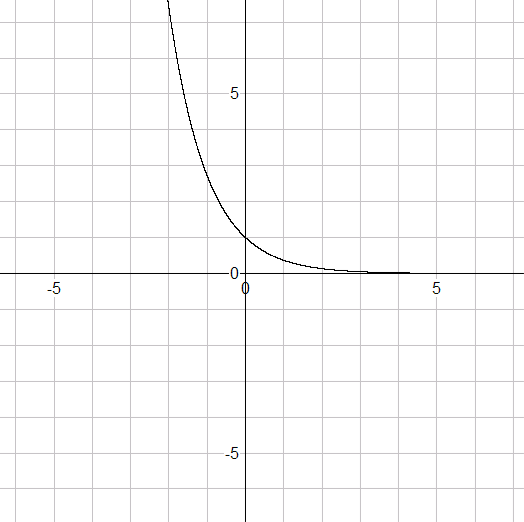
\includegraphics[ width=2.4336in, height=2.1241in,]{L4SZ2830}
}
\end{tabular} 


\begin{tabular}[c]{ll}31. The given graph is $y =e^{x}\text{.}$Draw $y =e^{x -2}$  &  \\
   
\setlength\fboxrule{0.01in}\setlength\fboxsep{0.2in}\fcolorbox[HTML]{000000}{FFFFFF}{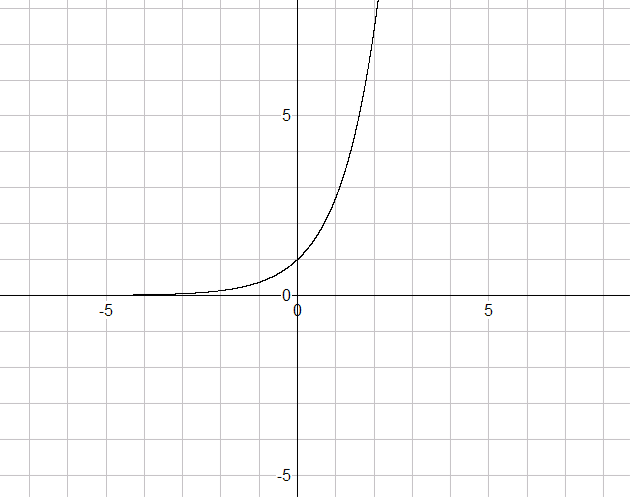
\includegraphics[ width=3.109in, height=2.4587in,]{L4SZ2831}
}
& 
\end{tabular}


\begin{description}
\item [43.] A radioactive substance decays in such a way that the amount
of mass remaining after $t$ days is given by the function
\begin{equation*}m (t) =13 e^{ -0.015 t}
\end{equation*} \\\relax Where $m (t)$ is measured in kilograms. 

\item [(a)]
Find the mass at time $t =0.$ 

\item [(b)] How much of the mass
remains after 45 days? 

\item [45.] A sky diver jumps from
a reasonable height above the ground. The air resistance she experiences is proportional to her velocity, and
the constant of proportionality is $0.2$. It can be shown that the downward velocity of the sky diver at time $t$ is given by
\begin{equation*}v (t) =80 \left (1 -e^{ -0.2 t}\right )
\end{equation*} \\\relax where $t$ is measured in seconds and $v (t)$ is measured in feet per second ($\mbox{ft}$/$\mbox{s}$). 

\item [(a)]
Find the initial velocity of the sky diver. 

\item [(b)] Find
the velocity after $5 \mbox{s}$ and after $10 \mbox{s}$. 

\item [(c)]
Draw a graph of the velocity function $v (t)\text{.}$ 

\item [(d)] The maximum
velocity of a falling object with wind resistance is called the \emph{terminal velocity}. From
the graph in part (c) find the terminal velocity of the sky diver. 

\item [48.]
The population of a certain species of bird is limited by the type of habitat required for nesting. The population
behaves according to the \emph{logistic growth model}
\begin{equation*}n (t) =\frac{5600}{0.5 +27.5 e^{ -0.044 t}}
\end{equation*} \\\relax where $t$ is measured in years. 

\item [(a)]
Find the initial bird population. 

\item [(b)] Draw a graph
of the function $n (t)\text{.}$ 

\item [(c)] What size does
the population approach as time goes on? \end{description}

 

\section{Logarithmic Functions}
The \emph{logarithmic function} is the inverse of the function $f (x) =a^{x}$. Recall the inverse of a function is the reflection of the function in the line $y =x$. Mathematically this is equivalent to swapping the $x$ and the y in $y =a^{x}$. So $x =a^{y}$ is the inverse of $y =a^{x}$. We have another notation for the inverse of a function, which is a little more complicated.
\ let $y =f (x)$ be a function of $x$ then $y =f^{ -1} (x)$ is the inverse of this function. Sometimes the inverse of the function is also a function.
\ For example the inverse of $y =x^{2}$ is $x =y^{2}$. $y =x^{2}$ is a function (vertical line test always applies), whereas $x =y^{2}$ is not a function (vertical line test is broken). 

   
\setlength\fboxrule{0.01in}\setlength\fboxsep{0.2in}\fcolorbox[HTML]{000000}{FFFFFF}{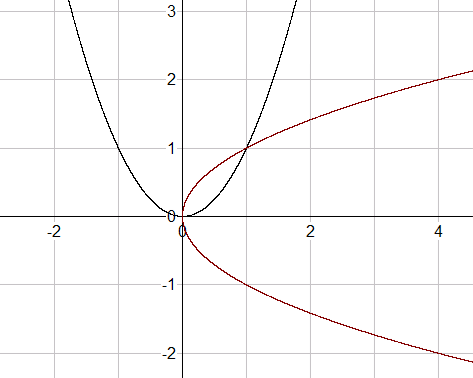
\includegraphics[ width=3.032in, height=2.4275in,]{L4SZ2832}
}


The inverse of $y =10^{x}$ is $x =10^{y}$. $y =10^{x}$ is a function (vertical line test always applies) and so is $x =10^{y}$. 

   
\setlength\fboxrule{0.01in}\setlength\fboxsep{0.2in}\fcolorbox[HTML]{000000}{FFFFFF}{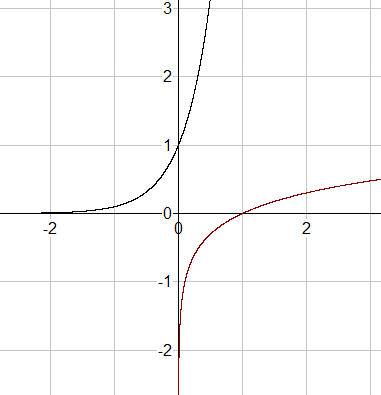
\includegraphics[ width=2.3419in, height=2.4267in,]{L4SZ2833}
}


Another useful fact to remember about inverses concerns the domain and range. The \emph{domain}
of $f$ is the \emph{range} of $f^{ -1}$ and the \emph{range} of $f$ is the \emph{domain} of $f^{ -1}$. 

We have a notation for $x =a^{y}$ it is $y =\log _{a} x$
\begin{equation}y =\log _{a} x \Leftrightarrow x =a^{y}\tag{1}
\end{equation}

In $x =a^{y}$ substitute $y =\log _{a} x$ and we get $x =a^{\log _{a} x}$. This means that given a base of $a$ the power (or exponent) to which $a$ must be raised to get $x$ is $\log _{a} x$. 

Problems involving logarithms will often require us to switch back and forth between $y =\log _{a} x$ and $x =a^{y}$, however it is also helpful if you can remember to substitute for $y$ and write $x =a^{\log _{a} x}$ so that you can say "the logarithm is the power". 

\subsubsection{Example 1}
\begin{description}
\item [(a)] $\log _{10} 100 =2$ because $10^{2} =100$ 

\item [(b)] $\log _{3} 81 =4$ because $3^{4} =81$ 

\item [(c)] $\log _{10} 0.01 = -2$ because $10^{ -2} =0.01$ \end{description}

\subsection{The graph of $y =\log _{a} x$}
The exponential function $y =a^{x}$ where $a >0$ is now known and its domain is $\mathbb{R}$ and its range is the positive real numbers. We often
write $\mathbb{R}^{ +}$ instead of $\left (0 ,\infty \right )$. 

The graph of $f (x) =a^{x}$ can be reflected in the line $y =x$ and the result is $f^{ -1} (x) =\log _{a} x$. 

\subsection{Graphing Exercise}


\subsubsection{Exercise 1}
On the same set of axes draw 


\begin{description}
\item [(a)] $y =10^{x}$ 

\item [(b)] $y =\log _{10} x$ 

\item [(c)] $y =x$ 

\item [(d)] $x =10^{y}$ \end{description}

Make a comment about each statement below. 

\begin{description}
\item [(1)] Check the graphs in (a), (b) and (c) are you confident that $y =\log _{10} x$ is the reflection of $y =10^{x}$ in the line $y =x$?\vspace{2cm} 

\item [(2)]
When you enter $x =10^{y}$ describe what takes place.\vspace{2cm} \end{description}

\subsubsection{Exercise 2}
On a \textbf{new} set of axes draw 


\begin{description}
\item [(a)] $y =2^{x}$ 

\item [(b)] $y =\log _{2} x$ \end{description}

There is no way to draw $y =\log _{2} x$ directly however (b) and (d) above gives you a way of doing it. 

\subsubsection{Exercise 3}
On a \textbf{new} set of axes draw 


\begin{description}
\item [(a)] $y =\log _{2} x$ 

\item [(b)] $y =\log _{3} x$ 

\item [(c)] $y =\log _{4} x$ 

\item [(d)] $y =\log _{5} x$ \end{description}

Notice the point that is common to all curves and the behaviour
of the family of curves for $x >1$ and for $0 <x <1$. 

\textbf{Property 1}: A property of logarithms is $\log _{a} 1 =0$ and this can be seen on the graphs where every graph goes through $\left (1 ,0\right )$. 

The pattern you observe as the base gets
bigger might not be evident for values of the base between $0$ and $1$. On the same set of axes draw the following: 


\begin{description}
\item [(e)] $y =\log _{\frac{1}{2}} x$ 

\item [(f)] $y =\log _{\frac{1}{3}} x$ 

\item [(g)] $y =\log _{\frac{1}{4}} x$ 

\item [(h)] $y =\log _{\frac{1}{5}} x$ \end{description}

To say the pattern is the same you have to be careful to describe
the base. Explain how changing the base gives the same pattern as for (a) to (d).


\textbf{Property 2:} A second property of logarithms is $\log _{a} a =1$. That is $a^{1} =a$ or the power to which you have to raise $a$ to get $a$ is $1$. On your curves above locate a point on each curve that shows this. You
should in each case be looking for the point $\left (a ,1\right )$. 

\textbf{Property 3:} A third property
of logarithms is $\log _{a} a^{x} =x$. This useful property must be understood if logarithm problems are to be mastered.
\ You should understand what $\log _{a} a^{x}$ is saying. $a$ is the base so $\log _{a} a^{x} =x$ says "The power to which $a$ must be raised to get $a^{x}$ is $x$." 

\subsection{Common Logarithms}
When the base is $10$ we write $y =\log _{10} x =\log  x$. If you see no base you assume it is base $10$. $y =\log  x$ is called the \emph{common} logarithm of $x$. Desmos and other programs with mathematics incorporated recognise "$\log $" as "logarithm to the base $10$". The $\log $ key on the calculator gives the common logarithm of any positive number.
\begin{equation*}y =\log  x \Leftrightarrow 10^{y} =x
\end{equation*}

\subsection{Natural Logarithms}
When the base is $e$ we write $y =\log _{e} x =\ln  x$. If you see $\ln  x$ you assume it is $\log _{e} x$. $y =\ln  x$ is called the \emph{natural} logarithm of $x$. Desmos and other programs with mathematics incorporated recognise "$\ln $" as "logarithm to the base $e$". The $\ln $ key on the calculator gives the natural logarithm of any positive number.
\begin{equation*}y =\ln  x \Leftrightarrow e^{y} =x
\end{equation*}

\subsection{Graphing Exercise}
Use Desmos to sketch the following. Describe in words how each curve is related to $y =\ln  x$. 


%TCIMACRO{\TeXButton{Begin 3 Columns}{\columnseprule =0pt
% \columnsep =30pt
% \begin {multicols}{3}}}%
%BeginExpansion
\columnseprule =0pt
\columnsep =30pt
\begin {multicols}{3}
%EndExpansion
 


\begin{description}
\item [(a)] $y =\ln  x$ 

\item [(b)] $y =\ln  ( -x)$ 

\item [(c)] $y = -\ln  x$ 

\item [(d)] $y =\ln  (x -1)$ 

\item [(e)] $y =\ln  (x) -1$ 

\item [(f)] $y =\ln  ( -1 -x)$ \end{description}


%TCIMACRO{\TeXButton{End 3 Columns}{\end {multicols}}}%
%BeginExpansion
\end {multicols}
%EndExpansion


\subsection{Exercises}
Express the equation in exponential form. 


\begin{tabular}[c]{lllllllllllll}1.  & (a)
& $\log _{5} 25 =2$  &  & (b)  & $\log _{5} 1 =0$  &  & 3.
& (a)  & $\log _{8} 2 =\frac{1}{3}$  &  & (b)  & $\log _{2} \genfrac{(}{)}{}{}{1}{8} = -3$  \\
5.  & (a)  & $\ln  5 =x$  &  & (b)  & $\ln  y =5$  &  &  &  &  &  &  & 
\end{tabular}

Express the equation in logarithmic form 


\begin{tabular}[c]{lllllllllllll}7.  & (a)
& $5^{3} =125$  &  & (b)  & $10^{ -4} =0.0001$  &  & 9.
& (a)  & $8^{ -1} =\frac{1}{8}$  &  & (b)  & $2^{ -3} =\frac{1}{8}$  \\
11.  & (a)  & $e^{x} =2$  &  & (b)  & $e^{3} =y$  &  &  &  &  &  &  & 
\end{tabular}

Evaluate the expression 


\begin{description}
\item [13. (a)]   
%TCIMACRO{\TeXButton{Begin 3 Columns}{\columnseprule =0pt
% \columnsep =30pt
% \begin {multicols}{3}}}%
%BeginExpansion
\columnseprule =0pt
\columnsep =30pt
\begin {multicols}{3}
%EndExpansion
 $\log _{3} 3$ 

\item [(b)] $\log _{3} 1$ 

\item [(c)] $\log _{3} 3^{2}$ 
%TCIMACRO{\TeXButton{End 3 Columns}{\end {multicols}}}%
%BeginExpansion
\end {multicols}
%EndExpansion
 

\item [15.
(a)]   
%TCIMACRO{\TeXButton{Begin 3 Columns}{\columnseprule =0pt
% \columnsep =30pt
% \begin {multicols}{3}}}%
%BeginExpansion
\columnseprule =0pt
\columnsep =30pt
\begin {multicols}{3}
%EndExpansion
 $\log _{6} 36$ 

\item [(b)] $\log _{9} 81$ 

\item [(c)] $\log _{7} 7^{10}$ 
%TCIMACRO{\TeXButton{End 3 Columns}{\end {multicols}}}%
%BeginExpansion
\end {multicols}
%EndExpansion
 

\item [17.
(a)]   
%TCIMACRO{\TeXButton{Begin 3 Columns}{\columnseprule =0pt
% \columnsep =30pt
% \begin {multicols}{3}}}%
%BeginExpansion
\columnseprule =0pt
\columnsep =30pt
\begin {multicols}{3}
%EndExpansion
 $\log _{3} \genfrac{(}{)}{}{}{1}{27}$ 

\item [(b)] $\log _{10} \sqrt{10}$ 

\item [(c)] $\log _{5} 0.2$ 
%TCIMACRO{\TeXButton{End 3 Columns}{\end {multicols}}}%
%BeginExpansion
\end {multicols}
%EndExpansion
 

\item [19.
(a)]   
%TCIMACRO{\TeXButton{Begin 3 Columns}{\columnseprule =0pt
% \columnsep =30pt
% \begin {multicols}{3}}}%
%BeginExpansion
\columnseprule =0pt
\columnsep =30pt
\begin {multicols}{3}
%EndExpansion
 $2^{\log _{2} 37}$ 

\item [(b)] $3^{\log _{3} 8}$ 

\item [(c)] $e^{\ln  \sqrt{5}}$ 
%TCIMACRO{\TeXButton{End 3 Columns}{\end {multicols}}}%
%BeginExpansion
\end {multicols}
%EndExpansion
 

\item [21.
(a)]   
%TCIMACRO{\TeXButton{Begin 3 Columns}{\columnseprule =0pt
% \columnsep =30pt
% \begin {multicols}{3}}}%
%BeginExpansion
\columnseprule =0pt
\columnsep =30pt
\begin {multicols}{3}
%EndExpansion
 $\log _{8} 0.25$ 

\item [(b)] $\ln  e^{4}$ 

\item [(c)] $\ln  \left (1/e\right )$ 
%TCIMACRO{\TeXButton{End 3 Columns}{\end {multicols}}}%
%BeginExpansion
\end {multicols}
%EndExpansion
 \end{description}

Use the definition of the logarithmic function to find $x$. 


\begin{description}
\item [23. (a)]   
%TCIMACRO{\TeXButton{Begin 4 Columns}{\columnseprule =0pt
% \columnsep =30pt
% \begin {multicols}{4}}}%
%BeginExpansion
\columnseprule =0pt
\columnsep =30pt
\begin {multicols}{4}
%EndExpansion
 $\log _{2} x =5$ 

\item [(b)] $\log _{2} 16 =x$ 

\item [25. (a)] $\log _{3} 243 =x$ 

\item [(b)] $\log _{3} x =3$ 
%TCIMACRO{\TeXButton{End 4 Columns}{\end {multicols}}}%
%BeginExpansion
\end {multicols}
%EndExpansion
 

\item [27.
(a)]   
%TCIMACRO{\TeXButton{Begin 4 Columns}{\columnseprule =0pt
% \columnsep =30pt
% \begin {multicols}{4}}}%
%BeginExpansion
\columnseprule =0pt
\columnsep =30pt
\begin {multicols}{4}
%EndExpansion
 $\log _{10} x =2$ 

\item [(b)] $\log _{5} x =2$ 

\item [29. (a)] $\log _{x} 16 =4$ 

\item [(b)] $\log _{x} 8 =\frac{3}{2}$ 
%TCIMACRO{\TeXButton{End 4 Columns}{\end {multicols}}}%
%BeginExpansion
\end {multicols}
%EndExpansion
 \end{description}

Find the domain of the function. 

\columnsep =30pt
\begin {multicols}{3}
\begin{description}
\item [57.] $f (x) =\log _{10} \left (x +3\right )$ 

\item [59.] $g (x) =\log _{3} \left (x^{2} -1\right )$ 

\item [61.] $h (x) =\ln  x +\ln  \left (2 -x\right )$ 
\end{description}\end {multicols}


\section{The Laws of Logarithms}
\begin{enumerate}
\item [Law 1] $\log _{a} \left (X Y\right ) =\log _{a} X +\log _{a} Y$ 

\item [Law 2] $\log _{a} \genfrac{(}{)}{}{}{X}{Y} =\log _{a} X -\log _{a} Y$ 

\item [Law 3] $\log _{a} X^{c} =c \log _{a} X$ 
\end{enumerate}


It is a useful exercise to prove these laws as the proofs show the
connection between the laws for exponents and the laws for logarithms. 

\textbf{Proof of law 1} \\\relax Let
$\log _{a} X =u$ so $a^{u} =X$ \\\relax and $\log _{a} Y =v$ so $a^{v} =Y$ \\\relax $X Y =a^{u} a^{v} =a^{u +v}$ \\\relax Take logarithms of both sides to the base $a$ \\\relax $\log _{a} X Y =\log _{a} a^{u +v} =u +v$ {\scriptsize (property 3)} $ =\log _{a} X +\log _{a} Y$ 

\textbf{Proof of law 2} \\\relax $\frac{X}{Y} =\frac{a^{u}}{a^{v}} =a^{u -v}$ \\\relax Take logarithms of both sides to the base $a$ \\\relax $\log _{a} \frac{X}{Y} =\log _{a} a^{u -v} =u -v$ {\scriptsize (property 3)} $ =\log _{a} X -\log _{a} Y$ 

\textbf{Proof of law 3} \\\relax $X^{c} =\left (a^{u}\right )^{c} =a^{u c} =a^{c u}$ \\\relax Take logarithms of both sides to the base $a$ \\\relax $\log _{a} X^{c} =\log _{a} a^{c u} =c u$ {\scriptsize (property 3)} $ =c \log _{a} X$ 

\subsubsection{Example 1}
Expand using the logarithm laws 


\begin{description}
\item [(a)] $\log  \sqrt{3} =\log  3^{\frac{1}{2}} =\frac{1}{2} \log  3$ 

\item [(b)] $\ln  \genfrac{(}{)}{}{}{a \sqrt{b}}{\sqrt[{3}]{c}} =\ln  \left (a b^{\frac{1}{2}} c^{ -\frac{1}{3}}\right ) =\ln  a +\ln  b^{\frac{1}{2}} +\ln  c^{ -\frac{1}{3}} =\ln  a +\frac{1}{2} \ln  b -\frac{1}{3} \ln  c$ \end{description}

\subsubsection{Example 2}
Evaluate 


\begin{description}
\item [(a)] $\log _{2} 112 -\log _{2} 7 =\log _{2} \frac{112}{7} =\log _{2} 16 =\log _{2} 2^{4} =4 \log _{2} 2 =4$ 

\item [(b)] $\log _{2} 8^{23} =\log _{2} \left (2^{3}\right )^{23} =\log _{2} \left (2^{69}\right ) =69 \log _{2} 2 =69$ 

\item [(c)] $\log  \sqrt{0.001} =\log  \left (0.001\right )^{\frac{1}{2}} =\frac{1}{2} \log  0.001 =\frac{1}{2} \log  10^{ -3} =\frac{1}{2} \times  -3 = -\frac{3}{2} = -1\frac{1}{2}$ 

\item [(d)] $e^{2 \ln  4} =\left (e^{\ln  4}\right )^{2} =4^{2} =16\text{\quad \quad }($Let $\ln  4 =x$ then $e^{x} =4$ so $e^{\ln  x} =4)$ \end{description}

\subsubsection{Example 3}
Rewrite as a single logarithm term using the logarithm laws 


\begin{description}
\item [(a)] $\log  12 +\frac{1}{2} \log  5 -\log  3 =\log  \frac{12 \sqrt{5}}{3} =\log  4 \sqrt{5}$ 

\item [(b)] $\log _{3} \left (x^{2} -1\right ) -\log _{3} \left (x -1\right ) =\log _{3} \frac{x^{2} -1}{x -1} =\log _{3} \frac{\left (x +1\right ) \left (x -1\right )}{x -1} =\log _{3} \left (x +1\right )$ \end{description}

\subsection{Exercises}
Use the Laws of Logarithms to rewrite the expression
in a form with no logarithms of products, quotients roots or powers. 


\begin{description}
\item [1.]   
%TCIMACRO{\TeXButton{Start 3 Columns}{\columnsep =30pt
% \begin {multicols}{3}}}%
%BeginExpansion
\columnsep =30pt
\begin {multicols}{3}
%EndExpansion
 $\log _{2} \left (2 x\right )$ 

\item [3.] $\log _{2} \left (x \left (x -1\right )\right )$ 

\item [5.] $\log  6^{10}$ 
%TCIMACRO{\TeXButton{End 3 Columns}{\end {multicols}}}%
%BeginExpansion
\end {multicols}
%EndExpansion
 

\item [7.]
%TCIMACRO{\TeXButton{Start 3 Columns}{\columnsep =30pt
% \begin {multicols}{3}}}%
%BeginExpansion
\columnsep =30pt
\begin {multicols}{3}
%EndExpansion
 $\log _{2} \left (A B^{2}\right )$ 

\item [9.] $\log _{3} \left (x \sqrt{y}\right )$ 

\item [11.] $\log _{5} \sqrt[{3}]{x^{2} +1}$ 
%TCIMACRO{\TeXButton{End 3 Columns}{\end {multicols}}}%
%BeginExpansion
\end {multicols}
%EndExpansion
 

\item [13.]
%TCIMACRO{\TeXButton{Start 3 Columns}{\columnsep =30pt
% \begin {multicols}{3}}}%
%BeginExpansion
\columnsep =30pt
\begin {multicols}{3}
%EndExpansion
 $\ln  \sqrt{a b}$ 

\item [19.] $\ln  \left (x \sqrt{\frac{y}{z}}\right )$ 

\item [21.] $\log  \sqrt[{4}]{x^{2} +y^{2}}$ 
%TCIMACRO{\TeXButton{End 3 Columns}{\end {multicols}}}%
%BeginExpansion
\end {multicols}
%EndExpansion
 \end{description}

Evaluate the expressions 


\begin{description}
\item [27.]   
%TCIMACRO{\TeXButton{Start 3 Columns}{\columnsep =30pt
% \begin {multicols}{3}}}%
%BeginExpansion
\columnsep =30pt
\begin {multicols}{3}
%EndExpansion
 $\log _{5} \sqrt{125}$ 

\item [29.] $\log  2 +\log  5$ 

\item [31.] $\log _{4} 192 -\log _{4} 3$ 
%TCIMACRO{\TeXButton{End 3 Columns}{\end {multicols}}}%
%BeginExpansion
\end {multicols}
%EndExpansion
 

\item [33.]
%TCIMACRO{\TeXButton{Start 3 Columns}{\columnsep =30pt
% \begin {multicols}{3}}}%
%BeginExpansion
\columnsep =30pt
\begin {multicols}{3}
%EndExpansion
 $\ln  6 -\ln  15 +\ln  20$ 

\item [35.] $10^{2 \log  4}$ 

\item [37.] $\log  \left (\log  1000^{10,000}\right )$ 
%TCIMACRO{\TeXButton{End 3 Columns}{\end {multicols}}}%
%BeginExpansion
\end {multicols}
%EndExpansion
 \end{description}

Rewrite the expression as a single logarithm 


\begin{description}
\item [39.]   
%TCIMACRO{\TeXButton{Start 3 Columns}{\columnsep =30pt
% \begin {multicols}{3}}}%
%BeginExpansion
\columnsep =30pt
\begin {multicols}{3}
%EndExpansion
 $\log _{3} 5 +5 \log _{3} 2$ 

\item [41.] $\log _{2} A +\log _{2} B -2 \log _{2} C$ 

\item [45.] $\ln  5 +2 \ln  x +3 \ln  \left (x^{2} +5\right )$ 
%TCIMACRO{\TeXButton{End 3 Columns}{\end {multicols}}}%
%BeginExpansion
\end {multicols}
%EndExpansion
 \end{description}

\section{Exponential and Logarithmic Equations}
The types of problems we meet in this section will be able to be rearranged so that they look like
\begin{equation*}a^{f (x)} =b
\end{equation*}

Where $a$ and $b$ are real numbers, $x$ is the unknown variable we are trying to find and $f (x)$ is an expression in $x$. The technique we will use will be the same for every problem we solve. 


\begin{description}
\item [Step 1] Our first step is to inspect the problem to see if the unknown
variable is in the exponent. 

\item [Step 2] Now that we have
established that we are solving an exponential equation we rearrange it until it is in the form $a^{f (x)} =b$ 

\item [Step 3] Take the logarithm
of both sides. In most practical situations we either take logarithms to the base $10$ or logarithms to the base $e$. there are three situations 

\item [Case
1] The problem has reduced to $10^{f (x)} =b$. Take logarithms to the base $10$. 

\item [Case 2] The problem has
reduced to $e^{f (x)} =b$. Take logarithms to the base $e$. 

\item [Case 3] The problem has
reduced to $a^{f (x)} =b$ where $a$ is neither $10$ nor $e$. You can take logarithms to the base $10$ or $e$ as you wish, either is correct. 

\item [Step 4]
Solve the equation you obtain. \end{description}

\subsubsection{Example 1}
Solve $3^{x} =5\text{\quad \quad }$This is an example of case $3$ above 

Take logarithms to the base $10$
\begin{align*}\log  3^{x} &  = \log  5 \\
x \log  3 &  = \log  5 \\
x &  = \frac{\log  5}{\log  3} \\
 &  \approx 1.464973521 \approx 1.46\text{(2 dp)}\end{align*}

Or take logarithms to the base $e$
\begin{align*}\ln  3^{x} &  = \ln  5 \\
x \ln  3 &  = \ln  5 \\
x &  = \frac{\ln  5}{\ln  3} \\
 &  \approx 1.464973521 \approx 1.46\text{(2 dp)}\end{align*}

This shows it is immaterial whether you take logarithms to the base $10$ or logarithms to the base $e$. 

\subsubsection{Example 2}
Solve $3^{2 x +1} =5$ 

Take logarithms to the base 10
\begin{align*}\log  3^{2 x +1} &  = \log  5 \\
\left (2 x +1\right ) \log  3 &  = \log  5 \\
2 x +1 &  = \frac{\log  5}{\log  3} \\
2 x &  = \frac{\log  5}{\log  3} -1 \\
x &  = \frac{1}{2} \left (\frac{\log  5}{\log  3} -1\right ) \\
 &  \approx 0.23248676 \approx 0.23\text{(2 dp)}\end{align*}

\subsubsection{Example 3}
Solve $4 \left (1 +10^{5 x}\right ) =9$ 

This must first be rearranged
\begin{align*}1 +10^{5 x} &  = \frac{9}{4} =2.25 \\
10^{5 x} &  = 2.25 -1 =1.25 \\
\text{}{\scriptsize 10}\text{}\log  10^{5 x} &  = \log  1.25 \\
5 x &  = \log  1.25 \\
x &  = \frac{1}{5} \log  1.25 \\
 &  \approx 0.019382002 \approx 0.019\text{(3 dp)}\end{align*}

\subsubsection{Example 4}
Solve $\frac{10}{1 +e^{ -x}} =3$
\begin{align*}1 +e^{ -x} &  = \frac{10}{3} \\
e^{ -x} &  = \frac{10}{3} -1 \\
 &  = \frac{10 -3}{3} =\frac{7}{3} \\
\text{}{\scriptsize e}\text{} -x &  = \ln  7 -\ln  3 \\
 &  \approx 0.84729786 \\
x &  \approx  -0.85\text{(2 dp)}\end{align*}

\subsection{Solving Logarithmic Equations}
Whereas exponential equations have the unknown variable in an exponent, logarithmic equations are equations containing the logarithm of an unknown
variable. 


\begin{description}
\item [Step 1] You recognise you are dealing with a logarithmic equation
by inspecting the problem to see if you have a logarithm of a term containing the unknown variable. 

\item [Step
2] Rearrange the equation until it is in the form
\begin{equation*}\log _{a} \left (\text{term containing unknown}\right ) =b
\end{equation*} \\\relax where $b$ is a number. 

\item [Step 3] Take
"antilogarithms". That is if $\log _{a} X =b$ then $a^{b} =X$ 

\item [Step 4] Solve the equation.
($a$ and $b$ are known and $X$ is an expression containing the unknown variable.) \end{description}

\subsubsection{Example 1}
Solve $\ln  x =5$ 

Take antilogarithms with base $e$.
\begin{align*}e^{5} &  = x \\
x &  \approx 148.4131591 \approx 148.4\text{(1 dp)}\end{align*}

\subsubsection{Example 2}
Solve $5 +4 \log  \left (5 x\right ) =17$
\begin{align*}4 \log  \left (5 x\right ) &  = 17 -5 =12 \\
\log  5 x &  = 3 \\
\text{}10^{3} &  = 5 x \\
x &  = \frac{1000}{5} =200\end{align*}

Check:\ Substitute $x =200$
\begin{align*}\text{LHS} &  = 5 +4 \log  \left (5 \times 200\right ) \\
 &  = 5 +4 \log  1000 =5 +4 \log  10^{3} \\
 &  = 5 +4 \times 3 =5 +12 =17 =\text{RHS}\end{align*}

\subsubsection{Example 3}
Solve $\log  x +\log  \left (x -1\right ) =\log  4 x$
\begin{align*}\log  x +\log  \left (x -1\right ) -\log  4 x &  = 0 \\
\log  \frac{x \left (x -1\right )}{4 x} &  = 0 \\
\log  \frac{1}{4} \left (x -1\right ) &  = 0 \\
\text{}10^{0} &  = \frac{1}{4} \left (x -1\right ) =1 \\
x -1 &  = 4 \\
x &  = 5\end{align*}

Check:
\begin{align*}\text{LHS} &  = \log  5 +\log  4 =\log  \left (5 \times 4\right ) =\log  20 \\
\text{RHS} &  = \log  4 \times 5 =\log  20 =\text{LHS}\end{align*}

\subsubsection{Example 4}
The velocity of a sky diver $t$ seconds after jumping is given by
\begin{equation*}v \left (t\right ) =80 \left (1 -e^{ -0.2 t}\right )
\end{equation*}

After how many seconds is the velocity $70$ $\mbox{ft}$/$\mbox{s}$?
\begin{align*}70 &  = 80 \left (1 -e^{ -0.2 t}\right ) \\
\frac{70}{80} &  = 1 -e^{ -0.2 t} \\
e^{ -0.2 t} &  = 1 -\frac{70}{80} \\
 &  = 1 -\frac{7}{8} =\frac{1}{8} =0.125 \\
\text{} -0.2 t &  = \ln  0.125 \\
t &  = \frac{\ln  0.125}{ -0.2} \approx 10.39\text{}\mbox{s}\end{align*}

\subsection{Exercises}
Find the solution of the exponential equation,
correct to four decimal places. 


\begin{description}
\item [1.]   
%TCIMACRO{\TeXButton{Start 3 Columns}{\columnsep =30pt
% \begin {multicols}{3}}}%
%BeginExpansion
\columnsep =30pt
\begin {multicols}{3}
%EndExpansion
 $e^{x} =16$ 

\item [3.] $10^{2 x} =5$ 

\item [5.] $2^{1 -x} =3$ 
%TCIMACRO{\TeXButton{End 3 Columns}{\end {multicols}}}%
%BeginExpansion
\end {multicols}
%EndExpansion
 

\item [7.]
%TCIMACRO{\TeXButton{Start 3 Columns}{\columnsep =30pt
% \begin {multicols}{3}}}%
%BeginExpansion
\columnsep =30pt
\begin {multicols}{3}
%EndExpansion
 $3 e^{x} =10$ 

\item [9.] $e^{1 -4 x} =2$ 

\item [11.] $4 +3^{5 x} =8$ 
%TCIMACRO{\TeXButton{End 3 Columns}{\end {multicols}}}%
%BeginExpansion
\end {multicols}
%EndExpansion
 

\item [13.]
%TCIMACRO{\TeXButton{Start 3 Columns}{\columnsep =30pt
% \begin {multicols}{3}}}%
%BeginExpansion
\columnsep =30pt
\begin {multicols}{3}
%EndExpansion
 $8^{0.4 x} =5$ 

\item [15.] $5^{ -x/100} =2$ 

\item [17.] $e^{2 x +1} =200$ 
%TCIMACRO{\TeXButton{End 3 Columns}{\end {multicols}}}%
%BeginExpansion
\end {multicols}
%EndExpansion
 

\item [19.]
%TCIMACRO{\TeXButton{Start 3 Columns}{\columnsep =30pt
% \begin {multicols}{3}}}%
%BeginExpansion
\columnsep =30pt
\begin {multicols}{3}
%EndExpansion
 $5^{x} =4^{x +1}$ 

\item [21.] $2^{3 x +1} =3^{x -2}$ 

\item [23.] $\frac{50}{1 +e^{ -x}} =4$ 
%TCIMACRO{\TeXButton{End 3 Columns}{\end {multicols}}}%
%BeginExpansion
\end {multicols}
%EndExpansion
 

\item [25.]
$100 \left (1.04\right )^{2 t} =300$ \end{description}

Solve the equations 


\begin{description}
\item [27.]   
%TCIMACRO{\TeXButton{Start Two Columns}{\columnsep =30pt
% \begin {multicols}{2}}}%
%BeginExpansion
\columnsep =30pt
\begin {multicols}{2}
%EndExpansion
 $x^{2} 2^{x} -2^{x} =0$ 

\item [29.] $4 x^{3} e^{ -3 x} -3 x^{4} e^{ -3 x} =0$ 
%TCIMACRO{\TeXButton{End Two Columns}{\end {multicols}}}%
%BeginExpansion
\end {multicols}
%EndExpansion
 

\item [31.]
%TCIMACRO{\TeXButton{Start Two Columns}{\columnsep =30pt
% \begin {multicols}{2}}}%
%BeginExpansion
\columnsep =30pt
\begin {multicols}{2}
%EndExpansion
 $e^{2 x} -3 e^{x} +2 =0$ 

\item [33.] $e^{4 x} +4 e^{2 x} -21 =0$ 
%TCIMACRO{\TeXButton{End Two Columns}{\end {multicols}}}%
%BeginExpansion
\end {multicols}
%EndExpansion
 \end{description}

Solve the logarithmic equations for $x$. 


\begin{description}
\item [35.]   
%TCIMACRO{\TeXButton{Start Two Columns}{\columnsep =30pt
% \begin {multicols}{2}}}%
%BeginExpansion
\columnsep =30pt
\begin {multicols}{2}
%EndExpansion
 $\ln  x =10$ 

\item [37.] $\log  x = -2$ 
%TCIMACRO{\TeXButton{End Two Columns}{\end {multicols}}}%
%BeginExpansion
\end {multicols}
%EndExpansion
 

\item [39.]
%TCIMACRO{\TeXButton{Start Two Columns}{\columnsep =30pt
% \begin {multicols}{2}}}%
%BeginExpansion
\columnsep =30pt
\begin {multicols}{2}
%EndExpansion
 $\log  \left (3 x +5\right ) =2$ 

\item [41.] $2 -\ln  \left (3 -x\right ) =0$ 
%TCIMACRO{\TeXButton{End Two Columns}{\end {multicols}}}%
%BeginExpansion
\end {multicols}
%EndExpansion
 

\item [43.]
%TCIMACRO{\TeXButton{Start Two Columns}{\columnsep =30pt
% \begin {multicols}{2}}}%
%BeginExpansion
\columnsep =30pt
\begin {multicols}{2}
%EndExpansion
 $\log _{2} 3 +\log _{2} x =\log _{2} 5 +\log _{2} \left (x -2\right )$ 

\item [45.] $\log  x +\log  \left (x -1\right ) =\log  \left (4 x\right )$ 
%TCIMACRO{\TeXButton{End Two Columns}{\end {multicols}}}%
%BeginExpansion
\end {multicols}
%EndExpansion
 

\item [47.]
%TCIMACRO{\TeXButton{Start Two Columns}{\columnsep =30pt
% \begin {multicols}{2}}}%
%BeginExpansion
\columnsep =30pt
\begin {multicols}{2}
%EndExpansion
 $\log _{5} \left (x +1\right ) -\log _{5} \left (x -1\right ) =2$ 

\item [49.] $\log _{9} \left (x -5\right ) +\log _{9} \left (x +3\right ) =1$ 
%TCIMACRO{\TeXButton{End Two Columns}{\end {multicols}}}%
%BeginExpansion
\end {multicols}
%EndExpansion
 

\item [51.]
For what value of $x$ is the following true? $\;\log  \left (x +3\right ) =\log  x +3$ 

\item [53.] Solve for $x$:\qquad $2^{2/\log _{5} x} =\frac{1}{16}$ 

\item [63.] A $15 \mbox{g}$ sample of radioactive iodine decays in such a way that the mass remaining
after $t$ days is given by $m \left (t\right ) =15 e^{ -0.087 t}$ where $m (t)$ is measured in grams. After how many days is there only $5 \mbox{g}$ remaining? 

\item [65.]
A small lake is stocked with a certain species of fish. The fish population is modelled by the function
\begin{equation*}P =\frac{10}{1 +4 e^{ -0.8 t}}
\end{equation*} \\\relax where $P$ is the number of fish in thousands and $t$ is measured in years since the lake was stocked. 

\item [(a)]
Find the fish population after $3$ years. 

\item [(b)] After how many
years will the fish population reach $5000$ fish? \end{description}


%TCIMACRO{\TeXButton{Start Two Columns}{\columnsep =30pt
% \begin {multicols}{2}}}%
%BeginExpansion
\columnsep =30pt
\begin {multicols}{2}
%EndExpansion
 


%TCIMACRO{\TeXButton{End Two Columns}{\end {multicols}}}%
%BeginExpansion
\end {multicols}
%EndExpansion

\clearpage
\section{Answers}
%TCIMACRO{\TeXButton{Start Two Columns}{\columnsep =30pt
% \begin {multicols}{2}}}%
%BeginExpansion
\columnsep =30pt
\begin {multicols}{2}
%EndExpansion
 

\textbf{Exercises 4.1} 

9. $f (x) =3^{x}$ 

10. $f (x) =5^{x}$ 

11. $f (x) =\genfrac{(}{)}{}{}{1}{4}^{x}$ 

12. $f (x) =\genfrac{(}{)}{}{}{1}{2}^{x}$ 

19. Use Desmos to verify. Plot $y = -(3^{x})$ 

21. Use Desmos to verify. 

23. Use Desmos to verify. 

25. Use Desmos to verify. Plot $y =10^{x +3}$ 

27. Use Desmos to verify. Plot $y = -(e^{x})$ 

29. Use Desmos to verify. 

31. Use Desmos to verify. 

43. (a)
$13 \mbox{kg}$ (b) $6.6 \mbox{kg}$ 

45. (a) $0$ (b) $50.6 ft/\mbox{s} ,69.2 ft/\mbox{s}$ (c) $ -$ (d) $80 ft/\mbox{s}$ 

48. (a) $200$ (b) $ -$ (c) $11,200$ 

\textbf{Exercises 4.2} 

1. (a) $5^{2} =25$ (b) $5^{0} =1$ 

3. $8^{1/3} =2$ (b) $2^{ -3} =\frac{1}{8}$ 

5. (a) $e^{x} =5$ (b) $e^{5} =y$ 

7. (a) $\log _{5} 125 =3$ (b) $\log _{10} 0.0001 = -4$ 

9. (a) $\log _{8} \frac{1}{8} = -1$ (b) $\log _{2} \frac{1}{8} = -3$ 

11. (a) $\ln  2 =x$ (b) $\ln  y =3$ 

13. (a) $1$ (b) $0$ (c) $2$ 

15. (a) $2$ (b) $2$ (c) $10$ 

17. (a) $ -3$ (b) $\frac{1}{2}$ (c) $ -1$ 

19. (a) $37$ (b) $8$ (c) $\sqrt{5}$ 

21. (a) $ -\frac{2}{3}$ (b) $4$ (c) $ -1$ 

23. (a) $32$ (b) $4$ 

25. (a) $5$ (b) $27$ 

27. (a) $100$ (b) $25$ 

57. $\left ( -3 ,\infty \right )$ 

59. $\left ( -\infty  , -1\right ) \cup \left (1 ,\infty \right )$ 

61. $\left (0 ,2\right )$ 

\textbf{Exercises 4.3} 

1.
$1 +\log _{2} x$ 

3. $\log _{2} x +\log _{2} \left (x -1\right )$ 

5. $10 \log  6$ 

7. $\log _{2} A +2 \log _{2} B$ 

9. $\log _{3} x +\frac{1}{2} \log _{3} y$ 

11. $\frac{1}{3} \log _{5} \left (x^{2} +1\right )$ 

13. $\frac{1}{2} \left (\ln  a +\ln  b\right )$ 

19. $\ln  x +\frac{1}{2} \left (\ln  y -\ln  z\right )$ 

21. $\frac{1}{4} \log  \left (x^{2} +y^{2}\right )$ 

27. $\frac{3}{2}$ 

29. $1$ 

31. $3$ 

33. $\ln  8$ 

35. $16$ 

37. $4 +\log  3$ 

39. $\log _{3} 160$ 

41. $\log _{2} \left (A B/C^{2}\right )$ 

45. $\ln  \left [5 x^{2} \left (x^{2} +5\right )^{3}\right ]$ 

\textbf{Exercises 4.4} 

1. $2.7726$ 

3. $0.3495$ 

5. $ -0.5850$ 

7. $1.2040$ 

9. $0.0767$ 

11. $0.2524$ 

13. $1.9349$ 

15. $ -43.0677$ 

17. $2.1492$ 

19. $6.2126$ 

21. $ -2.9469$ 

23. $ -2.4423$ 

25. $14.0055$ 

27. $ \pm 1$ 

29. $0 ,\frac{4}{3}$ 

31. $\ln  2 \approx 0.6931 ,0$ 

33. $\frac{1}{2} \ln  3 \approx 0.5493$ 

35, $e^{10} \approx 22026$ 

37. $0.01$ 

39. $\frac{95}{3}$ 

41. $3 -e^{2} \approx  -4.3891$ 

43. $5$ 

45. $5$ 

47. $\frac{13}{12}$ 

49. $51$ 

51. $\frac{3}{2}$ 

53. $1/\sqrt{5} \approx 0.4472$ 

63. $13$ days 

65. (a) $7337$ (b) $1.73 \mbox{y}$r 

\end {multicols}